%%%%%%%%%%%%%%%%%%%%%%%%%%%%%%%%%%%%%%%%%%%%%%%%%%%%%%%%%%%%%%%%%%%%%%%%%%%%%%%%
%2345678901234567890123456789012345678901234567890123456789012345678901234567890
%        1         2         3         4         5         6         7         8

\documentclass[letterpaper, 10 pt, conference]{ieeeconf}  % Comment this line out if you need a4paper

%\documentclass[a4paper, 10pt, conference]{ieeeconf}      % Use this line for a4 paper

\IEEEoverridecommandlockouts                              % This command is only needed if 
                                                          % you want to use the \thanks command

\overrideIEEEmargins                                      % Needed to meet printer requirements.

%In case you encounter the following error:
%Error 1010 The PDF file may be corrupt (unable to open PDF file) OR
%Error 1000 An error occurred while parsing a contents stream. Unable to analyze the PDF file.
%This is a known problem with pdfLaTeX conversion filter. The file cannot be opened with acrobat reader
%Please use one of the alternatives below to circumvent this error by uncommenting one or the other
%\pdfobjcompresslevel=0
%\pdfminorversion=4

% See the \addtolength command later in the file to balance the column lengths
% on the last page of the document

% The following packages can be found on http:\\www.ctan.org
%\usepackage{graphics} % for pdf, bitmapped graphics files
%\usepackage{epsfig} % for postscript graphics files
%\usepackage{mathptmx} % assumes new font selection scheme installed
%\usepackage{times} % assumes new font selection scheme installed
%\usepackage{amsmath} % assumes amsmath package installed
%\usepackage{amssymb}  % assumes amsmath package installed
\usepackage{algorithm}
\usepackage{algpseudocode}
\usepackage{graphicx}
\usepackage{url}
\usepackage{amsmath}
\usepackage{gensymb}

\title{\LARGE \bf
Computer Vision Informed Parameter Estimation
}

\author{
    Marc Hernandez$^{\dagger,1}$, Brair (Tilboon) Elberier$^{\dagger,1}$, and Ankur Mehta$^1$
    \thanks{$^{\dagger}$Co-primary authors with equal contribution.}
    \thanks{$^1$Laboratory for Embedded Machines and Ubiquitous Robots (LEMUR), Department of Electrical and Computer Engineering, University of California, Los Angeles, CA, 90095
    Email: \{\fontfamily{qcr}\selectfont{ \large marchernandez, tilboon, mehtank\}@ucla.edu}}
    \thanks{}
}


\begin{document}

\maketitle
\thispagestyle{empty}
\pagestyle{empty}


%%%%%%%%%%%%%%%%%%%%%%%%%%%%%%%%%%%%%%%%%%%%%%%%%%%%%%%%%%%%%%%%%%%%%%%%%%%%%%%%
\begin{abstract}
We propose a novel, computer vision (CV) informed parameter estimation pipeline, capable of generating parameter estimates for a prescribed linear dynamic system of interest, by (1) collecting a time-series of measurements via a state-of-the-art (SOTA) object detector, (2) quantitatively analyzing the physical behavior of an object throughout a time-series dataset, (3) hypothesizing the most likely parameter set based on our analysis of the system's motion profile. This analysis is then unified with the object detector's qualitative video analysis to refine an identified system's classification. We demonstrate these capabilities by recreating a common roadway scenario where a vehicle is recorded traversing a speed bump parallel to the camera lens. By observing the vehicle's reaction to the speed bump, we may collect measurements closely resembling the actual displacement of its suspension system. These measurements along with the prescribed Simple Harmonic Motion (SHM) model, enable the Multiple-Model Adaptive Estimation (MMAE) algorithm to estimate the most likely set of parameters that describes the real observed system. Using these estimations, we enhance the detector's classification of the vehicles by introducing a subcategory of \textit{perceived mass} that may be used by robotic, artificial intelligence (AI), and machine learning (ML) systems to enrich their understanding of an object's physical properties. Enabling said systems to make new inferences about the object's potential interactions with the environment. From the performed experiments, we observe an MAE of XX.XX\%,(Insert results here relating to our evaluation metrics) Github: \url{https://tinyurl.com/CVInformedParameterEstimation}
\end{abstract}


%%%%%%%%%%%%%%%%%%%%%%%%%%%%%%%%%%%%%%%%%%%%%%%%%%%%%%%%%%%%%%%%%%%%%%%%%%%%%%%%
\section{INTRODUCTION}
As robotics, artificial intelligence (AI), and machine learning (ML) continue to advance, new systems will be expected to handle increasingly complex tasks, that require a fundamental understanding of the qualitative and quantitative information contained in the observed environment.  Great strides have been made in the fields of robotics modeling, computer vision (CV), and natural language processing (NLP) by utilizing visual semantics, like \textit{color, shape,} and \textit{size} to classify, segment, and contextually analyze important content within time-series data to provide their systems with critical information enabling higher level functionality. However, when observing a system in motion, we may be capable of learning additional information about the system by also considering its spatiotemporal properties during analysis []. 

By observing a system's physical behavior over a sequence of time-series data, we can compare the behavior of probable system candidates, modeled after the ground truth system, against the ground truth data. Provided that the data accurately reflects the observed system's real-world behavior, we can leverage the physics-based information relayed by the systems motion profile to make estimations of intrinsic system parameters like \textit{mass, stiffness} and \textit{friction coefficient}. This quantitative analysis enhances understanding of the observed system and may allow external systems to refine their qualitative data obtained via semantic analysis. Traditionally, the methods required to obtain accurate estimations of intrinsic parameters, require specialized sensors that often necessitate considerable effort to scale or are difficult to incorporate into everyday scenarios. 

Building on previous work, we analyze vehicles traversing a speed bump, with and without passengers, recorded by a simple monocular camera setup. Specifically, we observe the motion of its suspension system in response to an input with various loads. From these observations, we generate a time-series dataset of measurements that closely reflects the displacement of the suspension system in an effort to estimate the vehicle's \textit{mass ($m$), spring constant ($k$)} and \textit{damping coefficient ($b$)} based on the given Simple Harmonic Motion (SHM) model. We leverage this qualitative analysis to refine the class assigned to the vehicle by introducing the subclassification of \textit{perceived load}, effectively fusing the qualitative and quantitative analysis.

In this study, we propose a CV-informed parameter estimation pipeline, that combines the strengths of semantic and physics-based analysis to enhance our understanding of observed linear dynamic systems in videos. We accomplish this by using a state-of-the-art (SOTA) object detection tool, to classify the type of system observed, in groups like \textit{Truck, SUV, Sports}, and to collect a history of time-series measurements of the system in motion. These measurements are then provided to the Multiple-Model Adaptive Estimation (MMAE) algorithm [4], to learn the most probable set of intrinsic parameters, based on its temporal properties, that describes the observed real system. From these newly learned system parameters, we develop a deeper understanding of the real system, that may enable external systems to generate new inferences that may have been indiscernible with semantics alone.

The contributions of this paper are summarized as follows:
\begin{itemize}
    \item A CV Informed Parameter Estimation pipeline \textit{(fig. 1)}, capable of ingesting and evaluating general linear dynamic systems subject to AWGN.
    \item A physics-based method of estimating a linear dynamic system's intrinsic parameters from observer data.
    \item A fused classification approach that leverages qualitative and quantitative data analysis to refine broad classification categories.
\end{itemize}

\begin{figure*}[h]
    \centering
    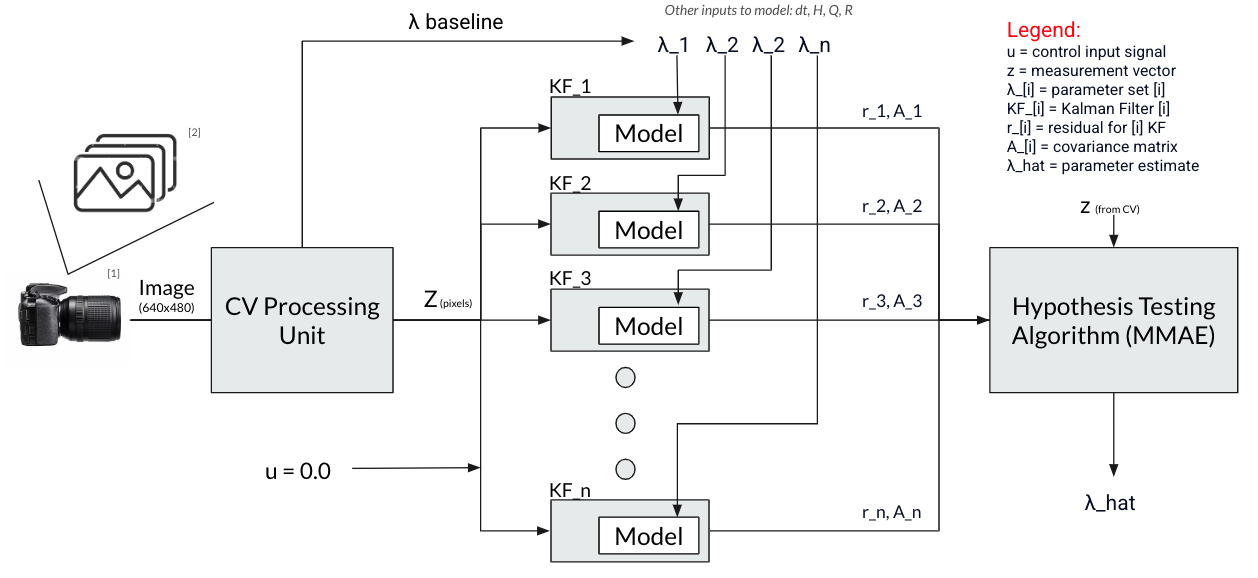
\includegraphics[width=\textwidth]{pipeline_diagram.png}
    \caption{CV Informed Parameter Estimation Pipeline}
    \label{figure_1}
\end{figure*}


\section{RELATED WORK}
(In progress) Existing works like [1], utilize CV to identify sidewall markings, record contact time and other mathematical relationships to derive an estimation of \textit{mass} for vehicles. However, the formulation of these methods, while accurate, are often limited in application scope and do not generalize to other parameters of interest.
Other works that generate affordances

\section{METHODOLOGY}
In the following section, we will closely examine the core components of our aforementioned pipeline, highlighting their requirements and influence on the pipeline's outcomes. 

\subsection{Object Detector}
Object detection is a well-studied and critical task in CV, enabling the automatic and accurate recognition of relevant visual features. In this study, employ a SOTA YOLOv11n [5] object detection model, pretrained on the COCO dataset, optimized on a custom dataset \url{https://tinyurl.com/CVIPEDataset}, and deployed using publicly available software packages [10] to localize and classify objects and their key-points captured in video frame data. The data augmentation strategies used during training were $\pm 10\%$ exposure and $\pm 10 \degree$ of horizontal and vertical image sheer. The resulting model achieved a mean Average Precision (mAP) over multiple intersection over union (IoU) of mAP50-95 $= 0.807$. In tandem with the defined model classes of \textit{Truck, SUV} and \textit{Sport} vehicles, we've associated each class with a statistical average mass $m$ in kg based on the entries of a large vehicle data found \url{https://carsheet.io/} to act the initial prediction for the remaining pipeline components.

\subsection{Kalman Filter Derivation}
The Kalman filter serves as the fundamental building block of the Multiple-Model Adaptive Estimation (MMAE) algorithm. The plant is modeled as a linear system subject to additive white Gaussian noise (AWGN). Each system within the parameter estimation pipeline is governed by a parameter vector $\lambda^k$, which is drawn from a predefined set of parameters derived from the CV identification process:

$$\Lambda = \{\lambda^1, \lambda^2, \dots, \lambda^k\}$$
These parameters define the dynamics of the system, where each $\lambda^k$ corresponds to a unique model hypothesis within the MMAE framework. To estimate the true system parameters, a bank of $k$ Kalman filters is maintained, each corresponding to a specific $\lambda^k$. The system associated with each estimator $k$ is governed by the following set of matrices:

$$\mathbf{S}^{k} = \{\mathbf{\Phi}(\lambda^{k}), \mathbf{B}(\lambda^{k}), \mathbf{H}^{k}, \mathbf{Q}^{k}, \mathbf{R}^{k}\}$$
These matrices define the following state-space equations associated with a particular hypothesized system (denoted by $k$) that form the basis of the Kalman filter.

$$
\mathbf{x}_{t_i}^{k} = \mathbf{\Phi}(\lambda^{k}) \mathbf{x}_{t_{i-1}}^{k} + \mathbf{B}(\lambda^{k}) \mathbf{u}_{t_{i-1}} + \mathbf{w}_{t_{i-1}}^{k} \eqno{(1)}
$$
$$
\mathbf{z}_{t_i}^{k} = \mathbf{H}^{k} \mathbf{x}_{t_i}^{k} + \mathbf{v}_{t_i}^{k} \eqno{(2)}
$$
The variables in these equations are defined as follows:
\vspace{0.25cm}
\begin{description}
    \item[$\mathbf{x}^{k}$] Kalman filter model state vector
    \item[$\mathbf{\Phi}(\lambda^{k})$] Kalman filter model state transition matrix
    \item[$\mathbf{B}(\lambda^{k})$] Kalman filter model control input matrix
    \item[$\mathbf{u}$] System input vector
    \item[$\mathbf{w}^{k}$] Kalman filter process noise input
    \item[$\mathbf{z}^{k}$] Kalman filter model measurement vector
    \item[$\mathbf{H}^{k}$] Kalman filter model output matrix
    \item[$\mathbf{v}^{k}$] Kalman filter measurement noise input
\end{description}
\vspace{0.25cm} 
It is important to note that the process noise $w^k$ and the measurement noise $v^k$ are independently drawn from zero mean, white Gaussian normal distributions and covariance defined by the matrices $Q$ and $R$, respectively.

$$\mathbf{w}_{t_{i-1}}^{k} \sim \mathcal{N}(0, \mathbf{Q}^k), \quad \mathbf{v}_{t_i}^{k} \sim \mathcal{N}(0, \mathbf{R}^k)$$
The derivation of these equations and the founding theory behind the Kalman filter are widely explored in these sources [4, 6, 7]. The following is a summary of the derivation from [4].

Using the model defined above, the Kalman filter defines the time propagation and measurement update equations for both the state estimate and its covariance matrix. The state estimate propagation equation is given by:
$$
\mathbf{\hat{x}}^{k}(t_i^-) = \mathbf{\Phi}(\lambda^{k}) \mathbf{\hat{x}}^{k}(t_{i-1}^+) + \mathbf{B}(\lambda^{k}) \mathbf{u}(t_{i-1}) \eqno{(3)}
$$
$$
\mathbf{\hat{z}}^{k}(t_i^-) = \mathbf{H}^k \mathbf{\hat{x}}^{k}(t_i^-) \eqno{(4)}
$$
The variables in these equations are defined as follows:
\vspace{0.25cm}
\begin{description}
    \item[$(t_i^-)$] time before measurement update at $i^{th}$ sample
    \item[$(t_{i-1}^+)$] time after measurement update at $(i-1)$ sample
    \item[$\mathbf{\hat{x}}^{k}$] Kalman filter state estimate vector
    \item[$\mathbf{\hat{z}}^{k}(t_i^-)$] Kalman filter measurement vector estimate before available
\end{description}
\vspace{0.25cm}
State estimate covariance matrix propagation equation:
$$
\mathbf{P}^k(t_i^-) = \mathbf{\Phi}(\lambda^{k}) \mathbf{P}^k(t_{i-1}^+) \mathbf{\Phi}(\lambda^{k})^\top + \mathbf{G}^k \mathbf{Q}^k (\mathbf{G}^k)^\top \eqno{(5)}
$$
Each Kalman filter updates the state estimate using:
$$
\hat{\mathbf{x}}^k(t_i^+) = \hat{\mathbf{x}}^k(t_i^-) + \mathbf{K}^k(t_i) \mathbf{r}^k(t_i) \eqno{(6)}
$$
and the Kalman filter gain is defined as:
$$
\mathbf{K}^k(t_i) = \mathbf{P}^k(t_i) (\mathbf{H}^k)^\top \mathbf{A}^k(t_i)^{-1} \eqno{(7)}
$$
The residual covariance matrix $A^k$, computed by the Kalman filter, is given by:
$$
\mathbf{A}^k(t_i) = \mathbf{H}^k \mathbf{P}^k(t_i^-) (\mathbf{H}^k)^\top + \mathbf{R}^k \eqno{(8)}
$$
The residual vector (innovation) $\mathbf{r}^k$ from (6) representing the difference between the actual measurement (z) and Kalman filter predicted measurement, per model, is calculated:
$$
\mathbf{r}^k(t_i) = \mathbf{z}(t_i) - \mathbf{H}^k \hat{\mathbf{x}}^k(t_i^-) \eqno{(9)}
$$
Finally, the Kalman filter state estimate covariance matrix is updated through the following equation:
$$
\mathbf{P}^k(t_i^+) = \mathbf{P}^k(t_i^-) - \mathbf{K}^k(t_i) \mathbf{H}^k \mathbf{P}^k(t_i^-) \eqno{(10)}
$$

\subsection{Simple Harmonic Motion Model Derivation}
To use Kalman filtering for the estimation of dynamic properties, a physics-based model of the system in question must first be developed.

The objective of this work is to be able to identify attributes or affordances of vehicles within a scene using video footage, specifically through the analysis of temporal features of the object rather than semantics alone. The natural model for a car as it evolves over time is a simple harmonic motion (SHM) model.

A damped simple harmonic oscillator follows the following second-order differential equation [8]:

$$m \ddot{x} + b \dot{x} + k x = u \eqno{(11)}$$
where:
\vspace{0.25cm}
\begin{description}
    \item[$m$] is the mass of the object
    \item[$b$] is the dampening coefficient of the spring
    \item[$k$] is the spring constant
    \item[$x$] is the displacement
    \item[$\dot{x}$] is the velocity
    \item[$\ddot{x}$] is the acceleration
    \item[$u$] is an external force applied to the system
\end{description}
\vspace{0.25cm}
The state space form of this equation can be represented as:
$$\begin{bmatrix} \dot{x} \\ \ddot{x} \end{bmatrix} = \begin{bmatrix} 0 & 1 \\ -\frac{k}{m} & -\frac{b}{m} \end{bmatrix} \begin{bmatrix} x \\ \dot{x} \end{bmatrix} + \begin{bmatrix} 0 \\ \frac{1}{m} \end{bmatrix} u \eqno{(12)}$$
which forms the basis for the state estimate propagation equation (3), where:
$$\mathbf{\Phi} = \begin{bmatrix} 0 & 1 \\ -\frac{k}{m} & -\frac{b}{m} \end{bmatrix}, \quad \mathbf{B} = \begin{bmatrix} 0 \\ \frac{\Delta t}{m} \end{bmatrix}$$
To make this compatible with a discrete-time Kalman filter, Euler’s approximation can be used to discretize the systems so that finally:
$$\mathbf{\Phi} = \begin{bmatrix} 1 & \Delta t \\ -\frac{k}{m} \Delta t & 1-\frac{b}{m} \Delta t\end{bmatrix}, \quad \mathbf{B} = \begin{bmatrix} 0 \\ \frac{1}{m} \end{bmatrix}$$
Now, these matrices can be substituted back into (3) to allow the discrete-time SHM model to be used in the prediction step to update the state estimate recursively based on input measurements.

The parameter vector $\lambda^k$ represents the set of parameters for the $k^{th}$ Kalman filter in the bank of estimators used in the MMAE algorithm. Each $\lambda^k$ consists of three unique components, $\{m, k, b\}$, which define the resulting dynamics of the corresponding system and are used to update the parameter estimate of the true system being modeled.

\subsection{Multiple-Model Adaptive Estimation Algorithm}
The Multiple Model Adaptive Estimation (MMAE) algorithm, as described in [4], employs a bank of Kalman filters, each configured with a distinct parameter set to simulate the dynamics of a real system. The primary objective of the algorithm is to run these estimators in parallel, continuously comparing their state estimates with incoming measurements. A Bayesian prediction strategy is then applied to probabilistically weight the predictions of each Kalman filter based on their consistency with the observed data. This approach allows the algorithm to identify and emphasize the models that best describe the system's behavior. As a result, the MMAE framework not only produces a weighted estimate of the true system state but can also be extended to infer a weighted estimate of the underlying parameter vector [4, 9].

The MMAE algorithm and its direct derivation have been thoroughly explored in various sources, a couple examples are [4, 9]. A brief summary is provided in table 1 because it will be applied in simulations.

\begin{table}[h]
    \centering
    \small
    \renewcommand{\arraystretch}{1.5}
    \setlength{\tabcolsep}{4pt} % Adjust spacing
    \begin{tabular}{|c|}
        \hline
        \textbf{Key Equations in the MMAE Framework} \\
        \hline
        \begin{minipage}{0.95\linewidth} % Minipage keeps content wrapped within column
            \begin{equation} 
                f_{z(t_i) | \mathbf{h}^k, Z(t_{i-1})} (\mathbf{z}_i \mid \mathbf{h}^k, \mathbf{Z}_{i-1}) = \beta^k \exp\{\cdot\} 
                \tag{13}
            \end{equation}
            \centering \textit{Conditional probability density function of the measurement.}
        \end{minipage} \\
        \hline
        \begin{minipage}{0.95\linewidth}
            \begin{equation} 
                \beta^k = \frac{1}{(2\pi)^{m/2} |\mathbf{A}^k|^{1/2}} 
                \tag{14}
            \end{equation}
            \centering \textit{Normalization constant for the Gaussian density function.}
        \end{minipage} \\
        \hline
        \begin{minipage}{0.95\linewidth}
            \begin{equation} 
                \{ \cdot \} = \left\{ -\frac{1}{2} \mathbf({r^k})^T (t_i) \mathbf({A}^k)^{-1} \mathbf{r}^k (t_i) \right\} 
                \tag{15}
            \end{equation}
            \centering \textit{Exponent term in the Gaussian density function.}
        \end{minipage} \\
        \hline
        \begin{minipage}{0.95\linewidth}
            \begin{equation} 
                q^k (t_i) = \mathbf({r}^k)^T (t_i) \mathbf({A}^k)^{-1} \mathbf{r}^k (t_i) 
                \tag{16}
            \end{equation}
            \centering \textit{Scalar likelihood quotient.}
        \end{minipage} \\
        \hline
        \begin{minipage}{0.95\linewidth}
            \begin{equation} 
                p^k (t_i) = \Pr\{\mathbf{h} = \mathbf{h}^k \mid \mathbf{Z}(t_i) = \mathbf{Z}_i\} 
                \tag{17}
            \end{equation}
            \centering \textit{Conditional probability of a hypothesis.}
        \end{minipage} \\
        \hline
        \begin{minipage}{0.95\linewidth}
            \begin{equation} 
                p^k (t_i) = \frac{ f_{z(t_i) | \mathbf{h}^k, Z(t_{i-1})} (\mathbf{z}_i \mid \mathbf{h}^k, \mathbf{Z}_{i-1}) \cdot p^k (t_{i-1}) }
                {\sum\limits_{j=1}^{K} f_{z(t_i) | \mathbf{h}_j, Z(t_{i-1})} (\mathbf{z}_i \mid \mathbf{h}_j, \mathbf{Z}_{i-1}) \cdot p_j (t_{i-1}) } 
                \tag{18}
            \end{equation}
            \centering \textit{Recursive Bayesian update for the hypothesis probability.}
        \end{minipage} \\
        \hline
    \end{tabular}
    \caption{Summary of key equations in the MMAE algorithm}
    \label{tab:equations_summary}
\end{table}

These equations wholistically describe the mathematical formulation for the MMAE hypothesis testing algorithm. Multiple Kalman filters are ran in parallel to evaluate different hypotheses for system parameters. Overall, first likelihoods of each hypothesis are calculated given new measurements. Next, the hypotheses are normalized and scored based on residual errors. Lastly, the probability of each hypothesis are updated recursively using Bayes’ theorem.

\begin{algorithm}
\caption{CV Informed Multiple-Model Adaptive Estimation (MMAE) for Vehicle Parameter Estimation} 
\label{alg:mmae}
\begin{algorithmic}[1]
    \Require 
    \begin{itemize}
        \item Video stream from camera
        \item Pre-trained CV pipeline
        \item Bank of Kalman Filters $\{KF^k\}$, each initialized with a parameter set $\lambda^k = \{m^k, k^k, b^k\}$
    \end{itemize}
    \Ensure Estimated vehicle parameters $\hat{\lambda} = [\hat{m}, \hat{k}, \hat{b}]$
    
    \State \textbf{Step 1: Measurement Acquisition}
    \State Capture image frame from video stream.
    \State Process image using CV to extract vehicle type and position $z$.
    
    \State \textbf{Step 2: Model Selection}
    \State Determine corresponding parameter set $\lambda^k$ based on identified vehicle type.
    
    \State \textbf{Step 3: Kalman Filter Updates}
    \For{each estimator $KF^k$ in $\{KF^k\}$}
        \State Compute predicted measurement $\hat{z}^k$ (4).
        \State Compute residual $r^k$ (9).
        \State Update Kalman gain and state estimate using (7) and (8).
    \EndFor
    
    \State \textbf{Step 4: Likelihood Computation}
    \For{each model $k$}
        \State Compute likelihood $f_{z | h^k, Z}$ using Eq. (13).
        \State Compute normalized weight $\beta^k$ using Eq. (14).
        \State Compute likelihood quotient $q^k$ using Eq. (16).
    \EndFor
    
    \State \textbf{Step 5: Bayesian Probability Update}
    \State Compute updated hypothesis probabilities $p^k(t_i)$ using Eq. (18).
    
    \State \textbf{Step 6: Parameter Estimation}
    \State Compute weighted estimate of $\lambda$:
    \[
        \hat{\lambda} = \sum_{k=1}^{K} p^k(t_i) \lambda^k
    \]
    
    \State \textbf{Step 7: Iterate for Next $t_i$}
\end{algorithmic}
\end{algorithm}

\section{EXPERIMENTS}
Using a simple monocular camera setup and a common roadway speed bump \textit{(fig. 2)}, we validate the claims of our proposed methodology by observing and measuring the displacement of a vehicle's suspension system as it traverses the speed bump obstacle. Two note cards are used as markers and are placed vertically inline with the center of the nearest wheel hub at each strut location. We record the vehicle with its direction of motion parallel to the camera's lens, moving at a near-constant speed, and measure the centroid of each note card, wheel, and vehicle body as well as their respective widths and heights in pixels. Then, we compute the difference between each visible wheel and note card pair for the entire collection of time-series measurements to closely capture the actual displacement of the vehicle suspension system in response to the speed bump input. This process is performed in three distinct vehicle classes, carrying three different loads. Finally, we utilize these newly collected measurements with the algorithmic implementation defined above to identify the most probable set of parameters, distinguishing each experiment case based only on differences in physical behavior. We then use this collection of experiments to answer the following questions:

\begin{itemize}
\item Is our architecture capable of generalizing to systems of high complexity using a prescribed physics-based model?
\item Can we accurately estimate the parameters of the prescribed model based on ground truth values?
\item Do these parameter estimates enable us to generate new inferences that characterize an object's properties and potential interactions with the environment?
\end{itemize}

\begin{figure}[h]
    \centering
    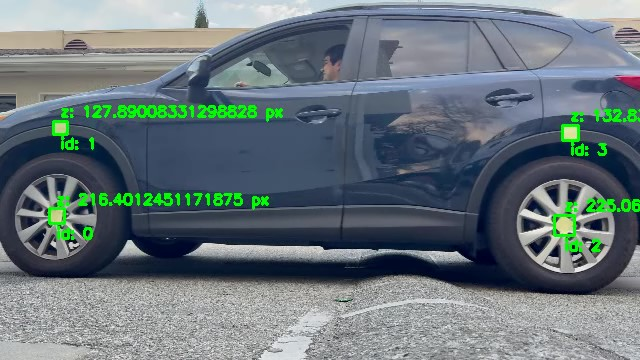
\includegraphics[width=\columnwidth]{4_points.jpg}
    \caption{Experiment Setup}
    \label{figure_2}
\end{figure}

\subsection {Test Cases}
We select the following vehicle classes: \textit{Truck, SUV,} and \textit{Sports}, due to their distinguishing system properties, allowing us to reinforce the claim of our pipeline architecture's generalizability, and testing each vehicle class under the following load configurations:
\begin{itemize}
    \item \textbf{Case A:} A driver, no passengers 
    \item \textbf{Case B:} A driver, two passengers
    \item \textbf{Case C:} A driver, four passengers
\end{itemize}

\subsection{Evaluation Metrics}
To evaluate the performance of the pipeline architecture, we utilize the following metrics to analyze the accuracy and fitment of our estimated parameters. 
\begin{itemize}
    \item \textbf{Mean Absolute Percentage Error (MAPE):} MAPE will be used to evaluate how close our forecast parameters are to the actual system parameters and is helpful in this situation due to its intuitive interpretation of the magnitude of relative error and is scale independent.
    $$\text{MAPE} = \frac{100}{N} \sum_{t=1}^{N} \left| \frac{z_t - \hat{z}_t}{z_t} \right|$$
    \item \textbf{Coefficient of Determination (R-squared):} The R-squared metric will be used to evaluate the quality of fit of our estimated parameters by measuring the proportion of variation in the measured model data, which is adjusted to account for the number of measurements $n$ and predictors $p$.
    $$R^2 = 1 - \frac{\sum_{t=1}^{n} (z_t - \hat{z}_t)^2}{\sum_{t=1}^{n} (z_t - \bar{z})^2}$$
    $$\text{Adjusted } R^2 = 1 - \left( \frac{(1 - R^2) \cdot (n - 1)}{n - p - 1} \right)$$
\end{itemize}

\section{RESULTS AND DISCUSSION}
(In progress) Here we discuss the results of our experiments


\section{FUTURE WORK}
(In progress)

Where can we take advantage of these newly generated affordances
a more sophisticated measurement device
discussion of the points Zida brought up -> embodied ai
\section{CONCLUSION}
In summary, this paper presents a CV-informed parameter estimation pipeline, an approach that capitalizes on qualitative and quantitative video data to classify objects and interpret intrinsic parameters to gain a holistic understanding of a subject of interest. Using this method we leverage the capabilities of the MMAE algorithm [4] by providing it with observational data from the CV processing unit that closely resembles the desired motion profile needed for analysis. From this evaluation, we're able to uncover... These results validate the contributions outlined in Section I, by...verifying the integrity of our results using synthetic and real-world testing...


\addtolength{\textheight}{-12cm}   % This command serves to balance the column lengths
                                  % on the last page of the document manually. It shortens
                                  % the textheight of the last page by a suitable amount.
                                  % This command does not take effect until the next page
                                  % so it should come on the page before the last. Make
                                  % sure that you do not shorten the textheight too much.

%%%%%%%%%%%%%%%%%%%%%%%%%%%%%%%%%%%%%%%%%%%%%%%%%%%%%%%%%%%%%%%%%%%%%%%%%%%%%%%%



%%%%%%%%%%%%%%%%%%%%%%%%%%%%%%%%%%%%%%%%%%%%%%%%%%%%%%%%%%%%%%%%%%%%%%%%%%%%%%%%



%%%%%%%%%%%%%%%%%%%%%%%%%%%%%%%%%%%%%%%%%%%%%%%%%%%%%%%%%%%%%%%%%%%%%%%%%%%%%%%%

\section*{ACKNOWLEDGMENT}
This study was supported by the Automated Domain-Understanding and Collaborative Agency (ADUCA) ECOLE project, started by a branch of General Electric (GE) in collaboration with the Laboratory for Embedded Machines and Ubiquitous Robots (LEMUR) lab.


%%%%%%%%%%%%%%%%%%%%%%%%%%%%%%%%%%%%%%%%%%%%%%%%%%%%%%%%%%%%%%%%%%%%%%%%%%%%%%%%

\begin{thebibliography}{99}
\bibitem{c1} M. Q. Feng, R. Y. Leung, and C. M. Eckersley, “Non-Contact vehicle Weigh-in-Motion using computer vision,” Redirecting, https://doi.org/10.1016/j.measurement.2019.107415. 
\bibitem{c2} G. E. Karniadakis et al., “Physics-informed Machine Learning,” Nature News, https://www.nature.com/articles/s42254-021-00314-5. 
\bibitem{c3} C. Meng, S. Seo, D. Cao, S. Griesemer, and Y. Liu, “When physics meets machine learning: A survey of physics-informed Machine Learning,” arXiv.org, https://doi.org/10.48550/arXiv.2203.16797.
\bibitem{c4} P. D. Hanlon and P. S. Maybeck, "Multiple-model adaptive estimation using a residual correlation Kalman filter bank," in IEEE Transactions on Aerospace and Electronic Systems, vol. 36, no. 2, pp. 393-406, April 2000, doi: 10.1109/7.845216.
\bibitem{c5} R. Khanam and M. Hussain, “Yolov11: An overview of the key architectural enhancements,” arXiv.org, https://doi.org/10.48550/arXiv.2410.17725. 
\bibitem{c6} R. E. Kalman, “A New Approach to Linear Filtering and Prediction Problems,” *Trans. ASME, J. Basic Eng.*, vol. 82, no. 1, pp. 35–45, Mar. 1960, doi: 10.1115/1.3662552.
\bibitem{c7} G. Welch and G. Bishop, “An Introduction to the Kalman Filter,” University of North Carolina, Tech. Rep. TR 95-041, 2001.
\bibitem{c8} P. Dourmashkin, “Chapter 23: Simple Harmonic Motion,” in \textit{Classical Mechanics}, Massachusetts Institute of Technology, MIT OpenCourseWare, 2016. [Online]. Available: \url{https://ocw.mit.edu/courses/8-01sc-classical-mechanics-fall-2016/pages/online-textbook/}. [Accessed: Mar. 5, 2025].
\bibitem{c9} D. Magill, "Optimal adaptive estimation of sampled stochastic processes," in \textit{IEEE Transactions on Automatic Control}, vol. 10, no. 4, pp. 434-439, Oct. 1965, doi: 10.1109/TAC.1965.1098191.
\bibitem{c10} Jocher, G., Qiu, J., \& Chaurasia, A. (2023). Ultralytics YOLO (Version 8.0.0) [Computer software]. https://github.com/ultralytics/ultralytics


\end{thebibliography}




\end{document}
